%!TEX ROOT = main.tex

\chapter{Results and Discussions}

\section{Introduction}
The results of the experiments are shown in this section. The differences in the accuracy and performance of each of the methods would be discussed and analysed. Hopefully, the results and discussions would be able to answer the research questions posted in the beginning of this research.

\section{The dataset}
\graphicspath{{./images/}}

\begin{figure} [ht]
\centering
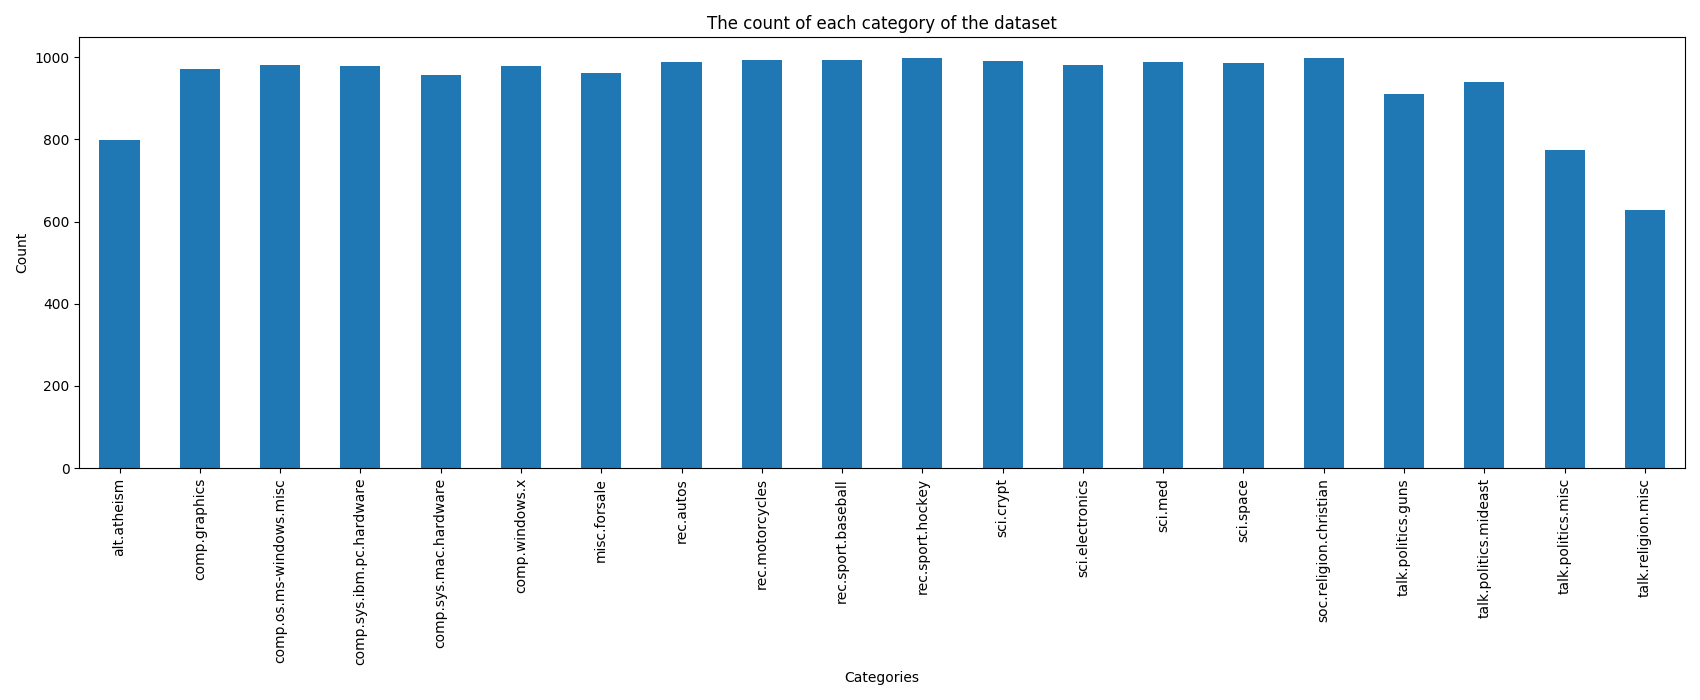
\includegraphics[width=\textwidth]{count}
\caption{The count of each category in the dataset}
\label{fig:freqCount}
\end{figure}

18790 rows, 15032 for training 3758 for testing
details about the 20news dataset, the category distributions, a table, a chart

\section{Term frequency}

\begin{table}[ht]
	\centering
	\begin{tabular}{|| c | c | c | c||}
		\hline
		ML & no of features & accuracy & time taken (s) \\ [0.5ex]
		\hline\hline
		kNN & 8000 & 0.28 & 3.65 \\ 
		\hline
		SVM & 8000 & 0.81 & 5.27 \\
		\hline
		NN & 8000 & 0.84 & 91.82 \\
		\hline
	\end{tabular}
\caption{Term frequency}
\label{tbl:termFrequency}
\end{table}

Term frequency is one of most common feature extraction method. It convert all the words in the dataset into a matrix where each column is a word and the rows are the number of times each word appear in the text. Each row in the matrix is a document. This vector space model representation of the words would result in a sparse matrix since each of the documents only contains a subset of all the words in the whole dataset. 

The number of features of the term frequency is limited to 8000, this is because of the memory constraint of the machine if it is unlimited the resulting matrix would be of bigger size and would have the probability of running out of memory while processing the matrix. 

In the results shown above, NN achieved an accuracy of 0.84 which is the best accuracy out of the 3 classification algorithm but it is also the one that takes the longest to process. kNN took the least time to process but has the lowest accuracy score. Performance wise SVM is the best, it only took 5s to process, which is 80s less than NN and has comparable accuracy with NN. 

reason of KNN accuracy low [reference] [https://arxiv.org/abs/1011.2807]
kNN accuracy is low in this scenario is possibly due to the feature matrix is sparse. The data points are few and far in between. kNN classify a new data point based on the distance of the new data point with the nearby data points. Since the other data points are few and sparse, the classification of the new data points would be biased. kNN is designed for low dimensional data therefore it doesn't perform well in large and sparse data.

\section{Term frequency with naive dimension reduction}

\begin{table} [ht]
	\centering
	\begin{tabular}{|| c | c | c | c | c||}
		\hline
		ML & parameter value & no of features & accuracy & time taken (s) \\ [0.5ex]
		\hline\hline
		kNN & 100 & 2530 & 0.27 & 4.16 \\ 
		\hline
		kNN & 500 & 478 & 0.32 & 4.88 \\ 
		\hline
		kNN & 1000 & 173 & 0.34 & 5.24 \\ 
		\hline\hline
		SVM & 7 & 15854 & 0.83 & 6.5 \\
		\hline
		SVM & 10 & 12705 & 0.83 & 6.58 \\
		\hline
		SVM & 100 & 2530 & 0.76 & 6.16 \\
		\hline\hline
		NN & 10 & 12705 & 0.87 & 116.78 \\
		\hline
		NN & 100 & 2530 & 0.80 & 48.08 \\
		\hline
		NN & 500 & 478 & 0.65 & 61.87 \\
		\hline\hline
	\end{tabular}
\caption{Term frequency with naive dimension reduction}
\label{tbl:termFrequencyNaive}
\end{table}

The feature extraction method used in this experiment is same as the experiment above but dimension reduction method is applied to the resulting matrix before training. The dimension reduction algorithm used in this experiment is a naive one which means that the columns with the least occurrence of word are removed.

The parameter value is just an integer value passed to the dimension reduction function implemented. It has an inversely proportional relationship with the number of features. The larger the parameter value, the more columns would be removed and the number of features would decrease.

In the result table above, each of the classification algorithm has different parameter value, this is determined by trial and error and the results shown are the best.

In this experiment, kNN still has the worst performance but its accuracy increases slightly as the number of features decreases and the time taken increases as well. SVM and NN have the same trend in this experiment, the accuracy and time taken decrease as the number of features decreases. This is because as the number of features decrease, there is less data to process thus the speedup and due to the decrease in training data, the model cannot correctly predict the test data.

In the scenarios where SVM and NN have more features than the experiment with just term frequency, both of the classification algorithms have better accuracy. These 2 classification algorithms are efficient and able to process features in a large and sparse vector space.



\section{Term frequency with SVD}

\begin{table} [ht]
	\centering
	\begin{tabular}{|| c | c | c | c||}
		\hline
		ML & no of features & accuracy & time taken (s) \\ [0.5ex]
		\hline\hline
		kNN & 2000 & 0.38 & 216.59 \\ 
		\hline
		kNN & 4000 & 0.31 & 482.66 \\
		\hline\hline
		SVM & 2000 & 0.78 & 172.58 \\
		\hline
		SVM & 4000 & 0.80 & 370.43 \\
		\hline\hline
		NN & 2000 & 0.79 & 91.13 \\
		\hline
		NN & 4000 & 0.8 & 220.76 \\
		\hline\hline
	\end{tabular}
\caption{Term frequency with SVD}
\label{tbl:termFrequencySvd}
\end{table}

In this experiment, the feature extraction method used is still term frequency but the dimension reduction algorithm changed. Instead of reducing the dimension by the least term frequency, SVD is used. SVD would retrieve the features with maximum variance in the data.

The number of features shown in the table above is the number of columns in the resulting matrix after applying SVD. 

Similar with the trend in the previous experiment (term frequency with naive dimension reduction), the accuracy of kNN increases slightly when the features decreases but the resulting accuracy is still far from satisfactory. The accuracy of SVM and NN also have the same trend with the previous experiment, the accuracy decreases slightly when the number of features decreases. 

As expected the time taken to process the features decreases as the number of features decreases. However, in comparison with the time taken in the previous experiments, the time taken in this experiment is astoundingly high. SVD would be the culprit, dimension reduction comes at a cost which is processing power. To reduce or compress the features into a small dimension, a lot of calculation would be involve, this would take both time and processing power.

The resulting accuracy is not as good as just with term frequency. This is expected because the number of features decreased. The reduction in features may save some memory space but in order to achieve that more processing power and time would be needed.

\section{TF-IDF}

\begin{table} [ht]
	\centering
	\begin{tabular}{|| c | c | c | c||}
		\hline
		ML & no of features & accuracy & time taken (s) \\ [0.5ex]
		\hline\hline
		kNN & 8000 & 0.76 & 3.71 \\ 
		\hline
		SVM & 8000 & 0.87 & 2.39 \\
		\hline
		NN & 8000 & 0.88 & 55.82 \\
		\hline
	\end{tabular}
\caption{TF-IDF}
\label{tbl:tfidf}
\end{table}

A different approach in feature extraction is applied in this experiment. Instead of term frequency which only take the frequency of each word into account, the feature extraction method used here in TF-IDF. The main difference of this feature extraction method is that besides term frequency it also take the rarity of the words into account. If a term or word appear in high frequency but in many documents, this word may not be of importance or a meaningful feature. If a word appear rarely and only in a few documents, this word would have high importance and would be meaningful feature of the few documents.

With TF-IDF, kNN can achieved a satisfactory accuracy score of 0.76 even though the number of features in the resulting matrix of TF-IDF is the same with term frequency which is 8000. The vector space model of TF-IDF would not be as sparse as that of term frequency which is kNN is more suitable to be applied.

NN is still provide the highest accuracy score of 0.88 but the time taken also the longest at 55.82s.

SVM achieved an accuracy of 0.87 which is just 0.01 shy of what achieved by NN and the time taken is the lowest among the 3 which is 2.39s.

In comparison to the few experiments with term frequency, the accuracy and time taken of the 3 classification model improves. This prove that TF-IDF is a better feature extraction method for text.


\section{TF-IDF with naive dimension reduction}

\begin{table} [ht]
	\centering
	\begin{tabular}{|| c | c | c | c | c||}
		\hline
		ML & parameter value & no of features & accuracy & time taken (s) \\ [0.5ex]
		\hline\hline
		kNN & 50 & 4221 & 0.74 & 4.00 \\ 
		\hline
		kNN & 100 & 2530 & 0.71 & 4.11 \\ 
		\hline
		kNN & 500 & 478 & 0.49 & 5.15 \\ 
		\hline\hline
		SVM & 50 & 4221 & 0.86 & 2.58 \\
		\hline
		SVM & 100 & 2503 & 0.83 & 2.63 \\
		\hline
		SVM & 500 & 478 & 0.66 & 2.94 \\
		\hline\hline
		NN & 50 & 4221 & 0.85 & 38.80 \\
		\hline
		NN & 100 & 2530 & 0.83 & 34.28 \\
		\hline
		NN & 500 & 478 & 0.64 & 77.12 \\
		\hline\hline
	\end{tabular}
\caption{TF-IDF with naive dimension reduction}
\label{tbl:tfidfNaive}
\end{table}

Similar with the experiment with term frequency, naive dimension reduction is applied to the vector space model generated from TF-IDF. The trend over all the 3 machine learning models when the number of features decreases, the accuracy of the model decreases slightly and the time taken increases. The amount of information has become lesser, less information is available to train a comprehensive model, therefore the accuracy decreases.The dimension reduction even though is a naive one and less computing intensive still increases the time taken compared with just with TF-IDF. The more reduction is performed, the time taken would increase as well.

The accuracy achieve with TF-IDF with naive dimension reduction is still passable with kNN at 0.74 when the features reduced from 8000 to 4221. However, when the number of features reduced to 478, the accuracy is just at a measly 0.49 which is not satisfactory. SVM and NN also achieved comparable accuracy at 0.86 and 0.85 respectively in comparison with TF-IDF when the number of features are almost halved.

From the results of this experiment, it can be deduced that with naive dimension reduction, the number of features and memory needed to store the vector space model is reduced. With this reduced number of features, the classification models can still achieve comparable performance but would be at a slightly decreased capacity.

\section{TF-IDF with SVD}

\begin{table} [ht]
	\centering
	\begin{tabular}{|| c | c | c | c||}
		\hline
		ML & no of features & accuracy & time taken (s) \\ [0.5ex]
		\hline\hline
		kNN & 2000 & 0.58 & 208.64 \\ 
		\hline
		kNN & 4000 & 0.77 & 457.16 \\
		\hline\hline
		SVM & 2000 & 0.86 & 69.63 \\
		\hline
		SVM & 4000 & 0.87 & 189.32 \\
		\hline\hline
		NN & 2000 & 0.84 & 87.12 \\
		\hline
		NN & 4000 & 0.85 & 215.73 \\
		\hline\hline
	\end{tabular}
\caption{TF-IDF with SVD}
\label{tbl:tfidfSvd}
\end{table}

Finally, the last experiment is TF-IDF with SVD dimension reduction. Similar with experiments above with SVD, each of the machine learning models would be tested with 2 set of vector space model, each with different number of features, namely 2000 and 4000. To put it in perspective, the number of features without reduction is 8000. 

When the number of features are at 4000 which is halved, kNN still can produced an accuracy of 0.77 which is similar with what is achieved with TF-IDF without dimension reduction. Same goes to SVM and NN, at 4000 features, the accuracy are quite similar with TF-IDF without dimension reduction. When the dimension of the vector space model is reduced to 2000, the accuracy across 3 of the classification models dropped. kNN being the most drastic, its accuracy dropped to 0.58 while SVM and NN dropped to 0.86 and 0.84 respectively, which is slightly worse than before but it is still satisfactory. 

There is an odd trend on the time taken for all 3 classification models though. The time taken in this experiment is much higher than the experiment of TF-IDF without dimension reduction and TF-IDF with naive dimension reduction which is expected. SVD reduction would take more time as more calculation is performed. However, the time taken decreased when the further reduction is done, kNN take 457s to reduce the vector space model from 8000 to 4000 but just 208s to reduce the vector space model from 8000 to 2000. Keep in mind that the time recorded here includes the time taken for the classification model to predict the test dataset as well. This trend appear in SVM and NN as well. SVM took 189s to reduce 8000 to 4000 but 69s to reduce 8000 to 2000 while NN took 215s to reduce 8000 to 4000 and 87s to reduce 8000 to 2000. 

The decrement in time could be explained with the reduction of features, the time taken to process them also reduced therefore it provided a speedup. This speedup with the reduction of features came at a cost though, which is accuracy. For SVM and NN, the reduction in accuracy is meagre and would be logical to trade the slight accuracy with the speedup but in kNN the trade off would be lopsided.